\chapter{Propuesta de Solución}

El diagnóstico de las limitaciones actuales en la gestión de medios de la plataforma Picta establece el punto 
de partida para la concepción de una solución técnica integral. La transición hacia una arquitectura dirigida 
por eventos demanda la formalización de especificaciones y el modelado de requisitos mediante historias de usuario, 
permitiendo traducir las necesidades detectadas en funcionalidades concretas. Asimismo, la estructuración de un plan 
de entrega sustentado en estimaciones de esfuerzo objetivas, en conjunto con la selección estratégica de patrones arquitectónicos, 
garantiza que la propuesta sea no solo viable desde el punto de vista técnico, sino también plenamente integrable y escalable dentro 
del ecosistema tecnológico existente.

\section{Propuesta de solución}

Teniendo en cuenta que la necesidad de darle solución a las deficiencias de la plataforma es
inminente, este documento propone el desarrollo de un módulo que deberá integrarse al sistema que
actualmente se encuentra funcionando en producción. El módulo tendrá como objetivo ofrecer el servicio
de subida de multimedia a los servidores de Picta con una resistencia a errores que permita recuperar
el progreso de la subida en caso de cualquier situación inesperada, mientras mantiene el uso del
servicio limitado a las personas con los permisos necesarios para administrar un canal. Además,
mediante el desacoplamiento de la subida y el renderizado de videos, se logrará una alta reducción de
carga de trabajo del lado del cliente. Más formalmente se desea que la integración del módulo permita:

\begin{itemize}
  \item \textbf{Gestionar la lista de subida de videos:} El módulo debe brindar a la web la
  posibilidad de manipular los estados de cada subida de video por parte de un administrador de canal,
  dándole opciones de cambiar su estado a `en curso', `pausada', `cancelada' y mantener una
  persistencia de estos datos en el servidor a largo plazo.

  \item \textbf{Pausar subidas de forma arbitraria:} La web debe ser capaz gracias a las
  funcionalidades brindadas por el módulo de cambiar arbitrariamente al estado `pausada' cualquier
  subida que se encuentre `en curso'.

  \item \textbf{Reanudar subidas con estado `pausada':} Luego de cambiar el estado a `pausada', el
  módulo web debe permitirle al cliente autorizado reanudar el proceso desde el punto en que estaba
  antes de cambiar a ese estado, ya sea de forma automática al haber perdido comunicación con el
  servidor o manual al haber elegido arbitrariamente detener momentáneamente el proceso.

  \item \textbf{Persistir históricamente registros de subidas en estado `cancelada':} La web debe ser
  capaz de mostrarle al cliente autorizado todas las subidas con estado `cancelada' que haya
  registrado.

  \item \textbf{Procesar arbitrariamente metadatos de videos subidos al servidor S3:} El módulo web
  debe permitirle al usuario autorizado, luego de haber terminado la subida de un video al servidor
  S3, procesar del lado de la API los metadatos relacionados con el video en cuestión.

  \item \textbf{Listar videos sin metadatos aún asociados:} El sistema debe, gracias al módulo web,
  mostrarle al usuario autorizado una lista de videos ya subidos al servidor de MinIO S3 pero que aún
  no han sido renderizados con los metadatos necesarios.
\end{itemize}

\section{Posibles estados de una subida}

A continuación, se describe un diagrama de flujo orientado a los posibles estados que deberá poder
tomar una subida de videos según el nuevo módulo web:

\begin{figure}[htbp]
  \centering
  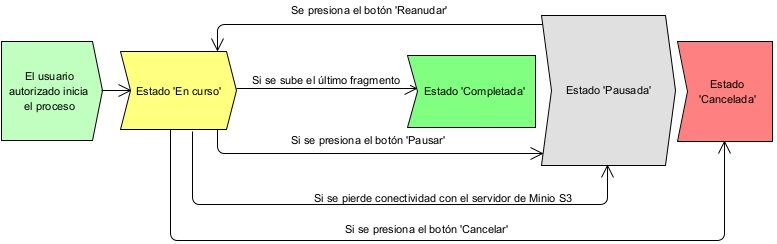
\includegraphics[width=0.95\textwidth]{Images/flujo_estados}
  \caption{Flujo de posibles estados de una subida. Elaboración propia}
  \label{fig:flujo_estados}
\end{figure}

A continuación, se describe un diagrama de flujo orientado a ilustrar la lógica que deberá tomar un
proceso de subida de videos según el nuevo módulo web:

\begin{figure}[htbp]
  \centering
  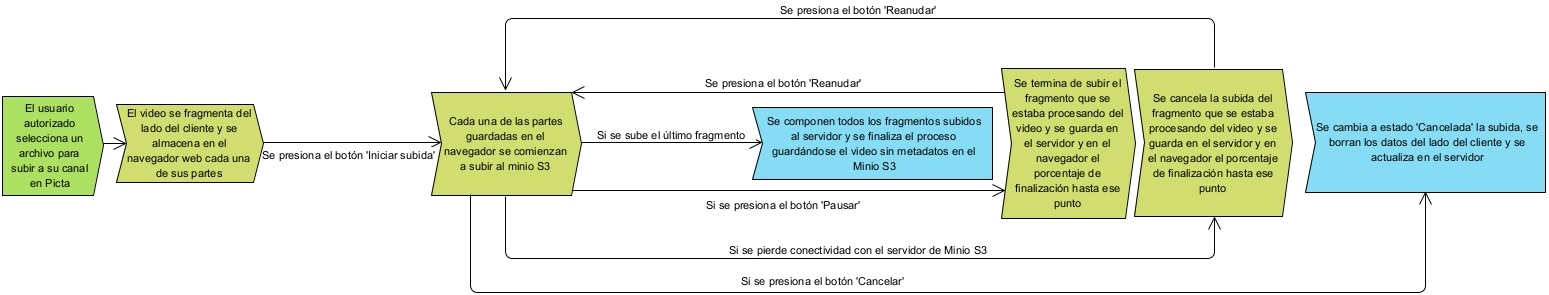
\includegraphics[width=0.95\textwidth]{Images/flujo_proceso}
  \caption{Flujo del proceso de subida de videos. Elaboración propia}
  \label{fig:flujo_proceso}
\end{figure}
 
\section{Historias de Usuario}

De acuerdo con \citep{Cohn2004}, las historias de usuario son uno de los principales
artefactos de desarrollo para los equipos de Scrum y Programación Extrema (XP). Una historia de
usuario es una definición de alto nivel de un requisito, que contiene la información justa para que
los desarrolladores puedan estimar razonablemente el esfuerzo necesario para implementarlo.

Como parte de la metodología Scrum se realizaron varias historias de usuario con el objetivo de tener
una mejor comprensión de los requisitos de la aplicación. A continuación, se presentan las historias
generadas.

\newcommand{\huhead}[4]{%
  \multicolumn{2}{|l|}{\colorentry{\textbf{Historia de Usuario}}} \\
  \hline
  \textbf{Número:} #1 \quad \textbf{Estimación:} #2 & \textbf{Sprint:} #3 \\
  \hline
  \multicolumn{2}{|p{13.5cm}|}{\textbf{Nombre:} #4} \\
  \hline
}

\newcommand{\huestereotipo}[3]{%
  % #1 = ruta de imagen, #2 = label, #3 = texto del caption
  \multicolumn{2}{|l|}{\textbf{Prototipo:}} \\
  \hline
  \multicolumn{2}{|p{13.5cm}|}{%
    \vspace{4pt}%
    \centering
    \includegraphics[width=0.75\linewidth]{#1}%
    \refstepcounter{figure}%
    \addcontentsline{lof}{figure}{\protect\numberline{\thefigure}#3}%
    \label{#2}%
    \par\smallskip
    {\small \textbf{Figura~\thefigure:} #3}%
    \vspace{4pt}%
  } \\
  \hline
}

% ── HU-01 ─────────────────────────────────────────────────────────────────────
\begin{longtable}[c]{|p{3.5cm}|p{10cm}|}
\caption{HU-01 Crear publicación y abrir popup de subida}
\label{tb:hu01}\\
\hline
\huhead{HU-01}{8 h}{1}{Crear publicación y abrir popup de subida}
\textbf{Prioridad de Negocio:} Crítica & \textbf{Asignado a:} Xavier Verdecie \\
\hline
\multicolumn{2}{|l|}{\textbf{Descripción:}} \\
\hline
\multicolumn{2}{|p{13.5cm}|}{Como administrador de canal de Picta, quiero poder crear una
publicación definiendo sus metadatos básicos (título, canal, categoría) y al guardar que se abra un
popup con una barra de progreso en 0\% con opciones para iniciar o cancelar la subida, para tener
control explícito sobre cuándo comienza la transferencia del archivo.} \\
\hline
\multicolumn{2}{|l|}{\textbf{Criterio de Aceptación:}} \\
\hline
\multicolumn{2}{|p{13.5cm}|}{\textbf{Given (Dado que):} El administrador de canal está autenticado y
accede al formulario de creación de publicación.} \\
\hline
\multicolumn{2}{|p{13.5cm}|}{\textbf{When (Cuando):} Completa los campos obligatorios (título, canal,
categoría, archivo de video) y presiona `Guardar'.} \\
\hline
\multicolumn{2}{|p{13.5cm}|}{\textbf{Then (Entonces):} Se registra la publicación en estado
`pendiente' y se muestra un popup modal con: barra de progreso en 0\%, botones `Iniciar' y
`Cancelar', y una cruz (X) arriba a la izquierda para cerrar y navegar a la página de gestión de
subidas.} \\
\hline
\multicolumn{2}{|l|}{\textbf{Validaciones:}} \\
\hline
\multicolumn{2}{|p{13.5cm}|}{\textbf{Frontend:} Validar campos obligatorios antes de permitir guardar.
Llamar a endpoint especializado para validar datos. El popup debe ser modal (bloquear interacción con
el fondo).\newline
\textbf{Backend:} Verificar token de sesión y permisos de administrador de canal antes de registrar la
publicación. Validar datos correctamente cuando se acceda al endpoint especializado.} \\
\hline
\multicolumn{2}{|l|}{\textbf{Observaciones:}} \\
\hline
\multicolumn{2}{|p{13.5cm}|}{Esta HU separa la creación de metadatos del inicio de la subida,
permitiendo al usuario revisar antes de comenzar la transferencia. La cruz del popup redirige
directamente a la página de gestión para facilitar el seguimiento de múltiples subidas.} \\
\hline
\huestereotipo{Images/Iniciar - Initial.jpg}{fig:hu01_estereotipo}{Prototipo de la HU-01:
  Interfaz del popup inicial de subida con barra de progreso en 0\% y botones Iniciar/Cancelar.
  Elaborado con Visual Paradigm como referencia visual.}
\end{longtable}

% ── HU-02 ─────────────────────────────────────────────────────────────────────
\begin{longtable}[c]{|p{3.5cm}|p{10cm}|}
\caption{HU-02 Iniciar proceso de carga fragmentada}
\label{tb:hu02}\\
\hline
\huhead{HU-02}{18 h}{1}{Iniciar proceso de carga fragmentada}
\textbf{Prioridad de Negocio:} Crítica & \textbf{Asignado a:} Xavier Verdecie \\
\hline
\multicolumn{2}{|l|}{\textbf{Descripción:}} \\
\hline
\multicolumn{2}{|p{13.5cm}|}{Como administrador de canal, quiero que al presionar `Iniciar' en el
popup de subida, el sistema divida el archivo en fragmentos y comience la transferencia de forma
controlada y tolerante a fallos de red, mostrando el progreso en tiempo real.} \\
\hline
\multicolumn{2}{|l|}{\textbf{Criterio de Aceptación:}} \\
\hline
\multicolumn{2}{|p{13.5cm}|}{\textbf{Given (Dado que):} El popup de subida está abierto con progreso
en 0\%.} \\
\hline
\multicolumn{2}{|p{13.5cm}|}{\textbf{When (Cuando):} El usuario presiona el botón `Iniciar'.} \\
\hline
\multicolumn{2}{|p{13.5cm}|}{\textbf{Then (Entonces):} El sistema registra una nueva sesión de subida
con estado `en curso', divide el archivo en fragmentos de tamaño configurable, calcula el checksum de
cada fragmento, comienza la transferencia secuencial al servidor MinIO S3, actualiza la barra de
progreso en tiempo real, y cambia los botones disponibles a `Pausar' y `Cancelar'.} \\
\hline
\multicolumn{2}{|l|}{\textbf{Validaciones:}} \\
\hline
\multicolumn{2}{|p{13.5cm}|}{\textbf{Frontend:} Deshabilitar el botón `Iniciar' una vez presionado.
Mostrar progreso por fragmento y global. Manejar errores de red con reintentos automáticos.\newline
\textbf{Backend:} Validar token de sesión. Cada fragmento recibido debe validarse con su checksum
(MD5/SHA256) \citep{Stallings2017} antes de almacenarse en MinIO. Rechazar solicitudes de roles sin
permisos.} \\
\hline
\multicolumn{2}{|l|}{\textbf{Observaciones:}} \\
\hline
\multicolumn{2}{|p{13.5cm}|}{Esta HU implementa el núcleo del protocolo de carga fragmentada sobre
Django REST Framework, utilizando minio-py v7.2.18. La lógica de partición reside en Angular v15.} \\
\hline
\huestereotipo{Images/Iniciar - Initial.jpg}{fig:hu02_estereotipo}{Prototipo de la HU-02:
  Popup de subida en curso mostrando progreso en tiempo real y botones Pausar/Cancelar.
  Elaborado con Visual Paradigm como referencia visual.}
\end{longtable}

% ── HU-03 ─────────────────────────────────────────────────────────────────────
\begin{longtable}[c]{|p{3.5cm}|p{10cm}|}
\caption{HU-03 Pausar subida de video en curso}
\label{tb:hu03}\\
\hline
\huhead{HU-03}{10 h}{1}{Pausar subida de video en curso}
\textbf{Prioridad de Negocio:} Alta & \textbf{Asignado a:} Xavier Verdecie \\
\hline
\multicolumn{2}{|l|}{\textbf{Descripción:}} \\
\hline
\multicolumn{2}{|p{13.5cm}|}{Como administrador de canal, quiero poder pausar una subida en curso
presionando el botón `Pausar' en el popup, para interrumpir temporalmente la transferencia sin perder
el progreso.} \\
\hline
\multicolumn{2}{|l|}{\textbf{Criterio de Aceptación:}} \\
\hline
\multicolumn{2}{|p{13.5cm}|}{\textbf{Given (Dado que):} Una subida está en curso con estado `en
curso'.} \\
\hline
\multicolumn{2}{|p{13.5cm}|}{\textbf{When (Cuando):} El usuario presiona `Pausar' en el popup.} \\
\hline
\multicolumn{2}{|p{13.5cm}|}{\textbf{Then (Entonces):} El frontend detiene el envío de nuevos
fragmentos, persiste el número del último fragmento enviado exitosamente, cambia el estado de la
sesión a `pausada', y actualiza los botones disponibles a `Reanudar' y `Cancelar'.} \\
\hline
\multicolumn{2}{|l|}{\textbf{Validaciones:}} \\
\hline
\multicolumn{2}{|p{13.5cm}|}{\textbf{Frontend:} Esperar confirmación del último fragmento en tránsito
antes de pausar. No permitir pausar si estado no es `en curso'. Si el navegador se cierra por algún
motivo o hay un timeout el proceso debe también cambiar al estado `pausada'.\newline
\textbf{Backend:} Validar que el usuario sea el propietario de la sesión.} \\
\hline
\multicolumn{2}{|l|}{\textbf{Observaciones:}} \\
\hline
\multicolumn{2}{|p{13.5cm}|}{La pausa arbitraria permite optimizar el uso del ancho de banda en
horarios de alto tráfico o liberar recursos temporalmente.} \\
\hline
\huestereotipo{Images/Pausar - Initial.jpg}{fig:hu03_estereotipo}{Prototipo de la HU-03:
  Popup con subida pausada mostrando botones Reanudar/Cancelar.
  Elaborado con Visual Paradigm como referencia visual.}
\end{longtable}

% ── HU-04 ─────────────────────────────────────────────────────────────────────
\begin{longtable}[c]{|p{3.5cm}|p{10cm}|}
\caption{HU-04 Reanudar subida pausada}
\label{tb:hu04}\\
\hline
\huhead{HU-04}{12 h}{1}{Reanudar subida pausada}
\textbf{Prioridad de Negocio:} Alta & \textbf{Asignado a:} Xavier Verdecie \\
\hline
\multicolumn{2}{|l|}{\textbf{Descripción:}} \\
\hline
\multicolumn{2}{|p{13.5cm}|}{Como administrador de canal, quiero poder reanudar una subida pausada
presionando el botón `Reanudar' en el popup, para continuar la transferencia desde el último fragmento
enviado exitosamente.} \\
\hline
\multicolumn{2}{|l|}{\textbf{Criterio de Aceptación:}} \\
\hline
\multicolumn{2}{|p{13.5cm}|}{\textbf{Given (Dado que):} Una subida está en estado `pausada'.} \\
\hline
\multicolumn{2}{|p{13.5cm}|}{\textbf{When (Cuando):} El usuario presiona `Reanudar' en el popup.} \\
\hline
\multicolumn{2}{|p{13.5cm}|}{\textbf{Then (Entonces):} El frontend consulta el último fragmento
registrado en el backend, reanuda la transferencia desde el siguiente fragmento, actualiza el estado a
`en curso', y cambia los botones disponibles a `Pausar' y `Cancelar'.} \\
\hline
\multicolumn{2}{|l|}{\textbf{Validaciones:}} \\
\hline
\multicolumn{2}{|p{13.5cm}|}{\textbf{Frontend:} Validar que todos los fragmentos previos al punto de
reanudación estén confirmados. Recalcular checksums de fragmentos no confirmados.\newline
\textbf{Backend:} Retornar el índice del último fragmento confirmado. Validar permisos de usuario.} \\
\hline
\multicolumn{2}{|l|}{\textbf{Observaciones:}} \\
\hline
\multicolumn{2}{|p{13.5cm}|}{Esta funcionalidad es crítica para la tolerancia a fallos de red y
desconexiones temporales del usuario.} \\
\hline
\huestereotipo{Images/Reanudar - Initial.jpg}{fig:hu04_estereotipo}{Prototipo de la HU-04:
  Popup reanudando una subida pausada desde el último fragmento confirmado.
  Elaborado con Visual Paradigm como referencia visual.}
\end{longtable}

% ── HU-05 ─────────────────────────────────────────────────────────────────────
\begin{longtable}[c]{|p{3.5cm}|p{10cm}|}
\caption{HU-05 Cancelar subida desde popup}
\label{tb:hu05}\\
\hline
\huhead{HU-05}{6 h}{1}{Cancelar subida desde popup}
\textbf{Prioridad de Negocio:} Media & \textbf{Asignado a:} Xavier Verdecie \\
\hline
\multicolumn{2}{|l|}{\textbf{Descripción:}} \\
\hline
\multicolumn{2}{|p{13.5cm}|}{Como administrador de canal, quiero poder cancelar una subida en cualquier
momento presionando el botón `Cancelar' en el popup, para detener definitivamente la transferencia y
cerrar el popup.} \\
\hline
\multicolumn{2}{|l|}{\textbf{Criterio de Aceptación:}} \\
\hline
\multicolumn{2}{|p{13.5cm}|}{\textbf{Given (Dado que):} Una subida está en cualquier estado excepto
`cancelada' o `completada'.} \\
\hline
\multicolumn{2}{|p{13.5cm}|}{\textbf{When (Cuando):} El usuario presiona `Cancelar' en el popup.} \\
\hline
\multicolumn{2}{|p{13.5cm}|}{\textbf{Then (Entonces):} El sistema detiene la transferencia, cambia el
estado de la sesión a `cancelada', cierra el popup y registra la subida cancelada en el historial.} \\
\hline
\multicolumn{2}{|l|}{\textbf{Validaciones:}} \\
\hline
\multicolumn{2}{|p{13.5cm}|}{\textbf{Frontend:} Solicitar confirmación antes de cancelar. Detener
cualquier operación de red activa.\newline
\textbf{Backend:} Validar permisos. Registrar timestamp de cancelación. No eliminar registros de la
base de datos.} \\
\hline
\multicolumn{2}{|l|}{\textbf{Observaciones:}} \\
\hline
\multicolumn{2}{|p{13.5cm}|}{Las subidas canceladas se mantienen en el historial para auditoría.} \\
\hline
\huestereotipo{Images/Pausar - Initial.jpg}{fig:hu05_estereotipo}{Prototipo de la HU-05:
  Confirmación de cancelación de subida en el popup.
  Elaborado con Visual Paradigm como referencia visual.}
\end{longtable}

% ── HU-06 ─────────────────────────────────────────────────────────────────────
\begin{longtable}[c]{|p{3.5cm}|p{10cm}|}
\caption{HU-06 Gestionar subidas en página dedicada}
\label{tb:hu06}\\
\hline
\huhead{HU-06}{16 h}{2}{Gestionar subidas en página dedicada}
\textbf{Prioridad de Negocio:} Alta & \textbf{Asignado a:} Xavier Verdecie \\
\hline
\multicolumn{2}{|l|}{\textbf{Descripción:}} \\
\hline
\multicolumn{2}{|p{13.5cm}|}{Como administrador de canal, quiero acceder a una página dedicada que
liste todas mis subidas con opciones para agrupar por nombre de video o estado, filtrar por `Todas',
`Sin procesar', `Procesadas', y ejecutar acciones específicas desde una columna `Acción', para tener
control centralizado sobre todas mis subidas.} \\
\hline
\multicolumn{2}{|l|}{\textbf{Criterio de Aceptación:}} \\
\hline
\multicolumn{2}{|p{13.5cm}|}{\textbf{Given (Dado que):} El administrador de canal está autenticado.} \\
\hline
\multicolumn{2}{|p{13.5cm}|}{\textbf{When (Cuando):} Navega a la página de gestión de subidas (ya sea
desde el botón de cruz del popup o desde el menú principal).} \\
\hline
\multicolumn{2}{|p{13.5cm}|}{\textbf{Then (Entonces):} Se muestra una lista de todas las subidas del
usuario con: agrupación configurable (por nombre de video o por estado), filtros (Todas, Sin procesar,
Procesadas), columnas con información relevante (video, estado), columna `Acción' con botones
contextuales según el estado (Iniciar, Pausar, Reanudar, Cancelar, Procesar, Ver, Eliminar), y la
capacidad de hacer clic en cualquier fila para abrir el popup de esa subida.} \\
\hline
\multicolumn{2}{|l|}{\textbf{Validaciones:}} \\
\hline
\multicolumn{2}{|p{13.5cm}|}{\textbf{Frontend:} Actualizar la lista en tiempo real cuando cambian
estados. Validar acciones permitidas según estado antes de mostrar botones. Implementar paginación
para listas grandes.\newline
\textbf{Backend:} Retornar únicamente subidas del usuario autenticado. Optimizar consultas con filtros
e índices.} \\
\hline
\multicolumn{2}{|l|}{\textbf{Observaciones:}} \\
\hline
\multicolumn{2}{|p{13.5cm}|}{Esta página centraliza toda la gestión de subidas. La columna `Acción'
muestra dinámicamente las operaciones válidas: cruz (X) para cancelar/eliminar según corresponda,
botones Iniciar/Pausar/Reanudar según estado de transferencia, botón Procesar para videos completados
sin procesar, y botón Ver para videos procesados.} \\
\hline
\huestereotipo{Images/Lista de subidas Bien - Initial.jpg}{fig:hu06_estereotipo}{Prototipo de
  la HU-06: Página de gestión de subidas con lista agrupable, filtrable y columna de acciones
  contextuales. Elaborado con Visual Paradigm como referencia visual.}
\end{longtable}

% ── HU-07 ─────────────────────────────────────────────────────────────────────
\begin{longtable}[c]{|p{3.5cm}|p{10cm}|}
\caption{HU-07 Completar subida y marcar como sin procesar}
\label{tb:hu07}\\
\hline
\huhead{HU-07}{8 h}{2}{Completar subida y marcar como sin procesar}
\textbf{Prioridad de Negocio:} Crítica & \textbf{Asignado a:} Xavier Verdecie \\
\hline
\multicolumn{2}{|l|}{\textbf{Descripción:}} \\
\hline
\multicolumn{2}{|p{13.5cm}|}{Como administrador de canal, quiero que cuando se termine de subir todos
los fragmentos de un video, el sistema cambie automáticamente el estado a `Completada | Sin Procesar'
y muestre la acción `Procesar' en la columna de acciones, para separar claramente la transferencia del
procesamiento de metadatos.} \\
\hline
\multicolumn{2}{|l|}{\textbf{Criterio de Aceptación:}} \\
\hline
\multicolumn{2}{|p{13.5cm}|}{\textbf{Given (Dado que):} Una subida está en estado `en curso' y se ha
enviado exitosamente el último fragmento.} \\
\hline
\multicolumn{2}{|p{13.5cm}|}{\textbf{When (Cuando):} El backend confirma la recepción y validación del
último fragmento mediante el endpoint `complete'.} \\
\hline
\multicolumn{2}{|p{13.5cm}|}{\textbf{Then (Entonces):} El sistema finaliza la sesión multipart en
MinIO, actualiza el estado a `completada' con sub-estado `sin\_procesar', cierra el popup si está
abierto, y en la página de gestión muestra los botones `Eliminar' (X) y `Procesar' en la columna
`Acción'.} \\
\hline
\multicolumn{2}{|l|}{\textbf{Validaciones:}} \\
\hline
\multicolumn{2}{|p{13.5cm}|}{\textbf{Frontend:} Actualizar la lista de gestión en tiempo real.\newline
\textbf{Backend:} Validar que todos los fragmentos estén confirmados antes de llamar a
`complete\_multipart\_upload' de MinIO. Actualizar timestamp de completado.} \\
\hline
\multicolumn{2}{|l|}{\textbf{Observaciones:}} \\
\hline
\multicolumn{2}{|p{13.5cm}|}{Este estado intermedio permite al usuario decidir cuándo procesar el
video, desacoplando la transferencia del procesamiento de metadatos y renderizado.} \\
\hline
\huestereotipo{Images/Lista de subidas sin publicar - Initial.jpg}{fig:hu07_estereotipo}{%
  Prototipo de la HU-07: Lista de gestión mostrando videos completados en estado ``Sin Procesar''
  con botón Procesar disponible. Elaborado con Visual Paradigm como referencia visual.}
\end{longtable}

% ── HU-08 ─────────────────────────────────────────────────────────────────────
\begin{longtable}[c]{|p{3.5cm}|p{10cm}|}
\caption{HU-08 Procesar video subido}
\label{tb:hu08}\\
\hline
\huhead{HU-08}{14 h}{2}{Procesar video subido}
\textbf{Prioridad de Negocio:} Crítica & \textbf{Asignado a:} Xavier Verdecie \\
\hline
\multicolumn{2}{|l|}{\textbf{Descripción:}} \\
\hline
\multicolumn{2}{|p{13.5cm}|}{Como administrador de canal, quiero poder presionar el botón `Procesar'
en un video con estado `Completada | Sin Procesar' para iniciar el procesamiento de metadatos y
transcodificación, y que el sistema gestione automáticamente los estados `Procesando', `En cola' o
`Fallido' según corresponda, hasta llegar a `Procesado' cuando termine exitosamente.} \\
\hline
\multicolumn{2}{|l|}{\textbf{Criterio de Aceptación:}} \\
\hline
\multicolumn{2}{|p{13.5cm}|}{\textbf{Given (Dado que):} Un video está en estado `Completada | Sin
Procesar'.} \\
\hline
\multicolumn{2}{|p{13.5cm}|}{\textbf{When (Cuando):} El usuario presiona el botón `Procesar' en la
columna `Acción'.} \\
\hline
\multicolumn{2}{|p{13.5cm}|}{\textbf{Then (Entonces):} El sistema valida que no haya otro video del
mismo usuario procesándose. Si no hay ninguno, cambia el estado a `Procesando' y envía un evento al
worker de Celery para iniciar el procesamiento asíncrono. Si hay otro procesándose, cambia el estado a
`En cola'. Durante el procesamiento, el worker actualiza el estado a `Fallida' si ocurre un error, o a
`Procesada' si termina exitosamente. Cuando un video llega a `Procesada', queda disponible en las
publicaciones del canal y el botón `Acción' cambia a `Ver' para navegar a la publicación.} \\
\hline
\multicolumn{2}{|l|}{\textbf{Validaciones:}} \\
\hline
\multicolumn{2}{|p{13.5cm}|}{\textbf{Frontend:} Deshabilitar el botón `Procesar' mientras se envía la
solicitud. Mostrar indicador de estado en tiempo real. Actualizar automáticamente cuando cambia de
`En cola' a `Procesando'.\newline
\textbf{Backend:} Validar permisos de usuario. Implementar lógica de cola FIFO para videos del mismo
usuario. El worker debe actualizar el estado en cada etapa del procesamiento (extracción de metadatos,
transcodificación, generación de miniaturas). Registrar logs detallados en caso de fallo.} \\
\hline
\multicolumn{2}{|l|}{\textbf{Observaciones:}} \\
\hline
\multicolumn{2}{|p{13.5cm}|}{El procesamiento asíncrono mediante Celery desacopla completamente la
carga pesada del servidor web. El sistema de cola garantiza que no se sobrecarguen los recursos con
múltiples transcodificaciones simultáneas. Los estados intermedios permiten al usuario hacer
seguimiento del progreso.} \\
\hline
\huestereotipo{Images/Lista de subidas sin publicar Monit - Initial.jpg}{fig:hu08_estereotipo}{%
  Prototipo de la HU-08: Lista de gestión mostrando videos en proceso de transcodificación con
  estados ``Procesando'', ``En cola'' o ``Fallida''. Elaborado con Visual Paradigm como referencia
  visual.}
\end{longtable}

% ── HU-09 ─────────────────────────────────────────────────────────────────────
\begin{longtable}[c]{|p{3.5cm}|p{10cm}|}
\caption{HU-09 Ver publicación de video procesado}
\label{tb:hu09}\\
\hline
\huhead{HU-09}{4 h}{2}{Ver publicación de video procesado}
\textbf{Prioridad de Negocio:} Baja & \textbf{Asignado a:} Xavier Verdecie \\
\hline
\multicolumn{2}{|l|}{\textbf{Descripción:}} \\
\hline
\multicolumn{2}{|p{13.5cm}|}{Como administrador de canal, quiero poder presionar el botón `Ver' en un
video con estado `Procesado' para navegar directamente a la página de la publicación, y verificar que
el video está disponible públicamente en el canal.} \\
\hline
\multicolumn{2}{|l|}{\textbf{Criterio de Aceptación:}} \\
\hline
\multicolumn{2}{|p{13.5cm}|}{\textbf{Given (Dado que):} Un video está en estado `Procesada'.} \\
\hline
\multicolumn{2}{|p{13.5cm}|}{\textbf{When (Cuando):} El usuario presiona el botón `Ver' en la columna
`Acción'.} \\
\hline
\multicolumn{2}{|p{13.5cm}|}{\textbf{Then (Entonces):} El sistema navega a la URL de la publicación
correspondiente y el video es reproducible.} \\
\hline
\multicolumn{2}{|l|}{\textbf{Validaciones:}} \\
\hline
\multicolumn{2}{|p{13.5cm}|}{\textbf{Frontend:} Abrir en nueva pestaña opcional.\newline
\textbf{Backend:} Validar que la publicación existe y está asociada al video procesado.} \\
\hline
\multicolumn{2}{|l|}{\textbf{Observaciones:}} \\
\hline
\multicolumn{2}{|p{13.5cm}|}{Esta funcionalidad cierra el ciclo permitiendo verificación inmediata
del resultado final.} \\
\hline
\huestereotipo{Images/Lista de subidas publicadas - Initial.jpg}{fig:hu09_estereotipo}{%
  Prototipo de la HU-09: Lista de gestión mostrando videos procesados con botón ``Ver'' para
  navegar a la publicación. Elaborado con Visual Paradigm como referencia visual.}
\end{longtable}

% ── HU-10 ─────────────────────────────────────────────────────────────────────
\begin{longtable}[c]{|p{3.5cm}|p{10cm}|}
\caption{HU-10 Eliminar registros de subidas}
\label{tb:hu10}\\
\hline
\huhead{HU-10}{6 h}{3}{Eliminar registros de subidas}
\textbf{Prioridad de Negocio:} Media & \textbf{Asignado a:} Xavier Verdecie \\
\hline
\multicolumn{2}{|l|}{\textbf{Descripción:}} \\
\hline
\multicolumn{2}{|p{13.5cm}|}{Como administrador de canal, quiero poder eliminar definitivamente
registros de subidas canceladas o completadas sin procesar desde la columna `Acción', para mantener
limpia mi lista de gestión de subidas.} \\
\hline
\multicolumn{2}{|l|}{\textbf{Criterio de Aceptación:}} \\
\hline
\multicolumn{2}{|p{13.5cm}|}{\textbf{Given (Dado que):} Un video está en estado `cancelada' o
`completada | sin\_procesar'.} \\
\hline
\multicolumn{2}{|p{13.5cm}|}{\textbf{When (Cuando):} El usuario presiona la cruz (X) en la columna
`Acción' y confirma la eliminación.} \\
\hline
\multicolumn{2}{|p{13.5cm}|}{\textbf{Then (Entonces):} El sistema elimina el registro de la base de
datos, elimina los fragmentos asociados del servidor MinIO (si los hay), y actualiza la lista de
gestión removiendo la entrada.} \\
\hline
\multicolumn{2}{|l|}{\textbf{Validaciones:}} \\
\hline
\multicolumn{2}{|p{13.5cm}|}{\textbf{Frontend:} Solicitar confirmación antes de eliminar. Mostrar
mensaje de éxito o error.\newline
\textbf{Backend:} Validar permisos. No permitir eliminación de videos en estado `procesando' o
`procesado'. Limpiar archivos asociados en MinIO.} \\
\hline
\multicolumn{2}{|l|}{\textbf{Observaciones:}} \\
\hline
\multicolumn{2}{|p{13.5cm}|}{La eliminación es irreversible y debe liberar espacio en MinIO.} \\
\hline
\huestereotipo{Images/Lista de subidas Bien - Initial.jpg}{fig:hu10_estereotipo}{%
  Prototipo de la HU-10: Lista de gestión con acción de eliminar disponible para subidas
  canceladas o sin procesar. Elaborado con Visual Paradigm como referencia visual.}
\end{longtable}

\section{Requisitos No Funcionales}

Los requisitos no funcionales (RNF) son esenciales para el desarrollo de software y determinan el
rendimiento de un sistema más allá de sus funciones básicas. Si bien los requisitos funcionales
especifican lo que un sistema debe hacer, los RNF definen qué tan bien debe
funcionar. Estos requisitos cubren aspectos críticos como el rendimiento, la seguridad, la facilidad
de uso y la escalabilidad, que afectan la confiabilidad del sistema, la experiencia del usuario y el
éxito a largo plazo \citep{Wiegers2013}.

Dado que el módulo se integra a una plataforma en producción con más de 700 canales activos y opera
bajo las restricciones de la infraestructura de red nacional, estos requisitos son determinantes para
garantizar la robustez, eficiencia e integrabilidad de la solución.

\subsection{Confiabilidad}

Dadas las limitaciones de conectividad del entorno nacional, la confiabilidad es el atributo de mayor
prioridad del sistema. El módulo debe garantizar que ninguna interrupción, ya sea de red o energía,
resulte en pérdida de progreso o datos para el usuario.

\begin{longtable}[c]{|p{1.8cm}|p{3cm}|p{8cm}|}
\caption{Requisitos de Confiabilidad}
\label{tb:rnf_confiabilidad}\\
\hline
\multicolumn{3}{|l|}{\colorentry{\textbf{Confiabilidad}}} \\
\hline
\textbf{ID} & \textbf{Requisito} & \textbf{Descripción} \\
\hline
\endfirsthead
\caption[]{Continuación de la página anterior} \\
\hline
\textbf{ID} & \textbf{Requisito} & \textbf{Descripción} \\
\hline
\endhead
\multicolumn{3}{r}{{Continúa en la próxima página}} \\
\endfoot
\hline
\endlastfoot

RnF-C1 & Persistencia ante interrupciones &
El sistema debe guardar automáticamente el progreso de cada carga fragmentada ante cualquier
interrupción de red o energía, tanto del lado del cliente como del servidor, garantizando la
reanudación sin pérdida de datos. \\ \hline

RnF-C2 & Manejo controlado de excepciones &
Cualquier error o excepción generada durante la subida o el renderizado debe ser capturada, registrada
internamente y comunicada al usuario con un mensaje descriptivo, evitando fallos silenciosos. \\ \hline

\end{longtable}

\subsection{Eficiencia}

El sistema debe mantenerse dentro de umbrales de rendimiento que no degraden la experiencia de los
creadores de contenido ni el desempeño general de la plataforma Picta.

\begin{longtable}[c]{|p{1.8cm}|p{3cm}|p{8cm}|}
\caption{Requisitos de Eficiencia}
\label{tb:rnf_eficiencia}\\
\hline
\multicolumn{3}{|l|}{\colorentry{\textbf{Eficiencia}}} \\
\hline
\textbf{ID} & \textbf{Requisito} & \textbf{Descripción} \\
\hline
\endfirsthead
\caption[]{Continuación de la página anterior} \\
\hline
\textbf{ID} & \textbf{Requisito} & \textbf{Descripción} \\
\hline
\endhead
\multicolumn{3}{r}{{Continúa en la próxima página}} \\
\endfoot
\hline
\endlastfoot

RnF-E1 & Tiempo de respuesta &
El tiempo de ejecución de cada transacción API no debe superar 1 segundo bajo condiciones normales de
operación de red. \\ \hline

RnF-E2 & Capacidad de procesamiento &
El sistema debe ser capaz de gestionar hasta 500 solicitudes de inicio de carga fragmentada por
segundo y soportar hasta 500 usuarios concurrentes sin degradación del rendimiento. \\ \hline

\end{longtable}

\subsection{Restricciones de Diseño e Implementación}

El módulo se desarrolla como una extensión del sistema existente de Picta, por lo que las decisiones
tecnológicas están condicionadas por la arquitectura actual. A continuación, se consolidan todas las
restricciones técnicas y de diseño que enmarcan el desarrollo.

\begin{longtable}[c]{|p{3cm}|p{10.3cm}|}
\caption{Restricciones de Diseño e Implementación}
\label{tb:restricciones}\\
\hline
\multicolumn{2}{|l|}{\colorentry{\textbf{Restricciones de Diseño e Implementación}}} \\
\hline
\textbf{Categoría} & \textbf{Especificación} \\
\hline
\endfirsthead
\caption[]{Continuación de la página anterior} \\
\hline
\textbf{Categoría} & \textbf{Especificación} \\
\hline
\endhead
\multicolumn{2}{r}{{Continúa en la próxima página}} \\
\endfoot
\hline
\endlastfoot

Almacenamiento &
La gestión de objetos multimedia se realiza exclusivamente mediante MinIO (librería minio-py v7.2.18),
compatible con la API de Amazon S3. \\ \hline

Base de datos &
PostgreSQL 17 como gestor de base de datos relacional. Administración mediante Navicat Premium
v17.1.10. \\ \hline

Modelado &
Visual Paradigm v17.0 para la generación de todos los artefactos UML del proyecto. \\ \hline

Codificación &
El código Python v3.9.6 debe adherirse al estándar PEP 8. Se deben aplicar buenas prácticas de diseño ágil
durante todo el desarrollo. \\ \hline

Interfaz &
La interfaz de usuario debe integrarse de forma seamless con el diseño visual existente de la
plataforma Picta, sin introducir inconsistencias estéticas. \\ \hline

Mantenimiento &
El sistema debe recibir revisiones periódicas para corregir errores e inconsistencias detectadas
durante su ciclo de vida en producción. \\ \hline

\end{longtable}

\section{Estimación de esfuerzo por historia de usuario y plan de iteraciones}

\citep{Pressman2014} señala que cumplir con los plazos y mantener la calidad son
fundamentales en el desarrollo de software, y que uno de los aspectos cruciales es la estimación del
tiempo.

En esta sección se presentan las estimaciones de esfuerzo de cada historia de usuario y el plan de
iteraciones derivado. Las horas declaradas en cada historia de usuario representan el esfuerzo de
implementación combinado de frontend y backend. Para convertirlas a semanas se considera una
dedicación efectiva de \textbf{10 horas semanales}, ritmo coherente con la carga académica
simultánea del desarrollador. La conversión se obtiene mediante la siguiente expresión:

\begin{table}[htbp]
\centering
\caption{Estimación de esfuerzo por historia de usuario}
\label{tab:estimacion}
\begin{tabular}{|c|l|c|c|}
\hline
\textbf{ID} & \textbf{Historia de Usuario} & \textbf{Estimación (h)} & \textbf{Sprint} \\
\hline
HU-01 & Crear publicación y abrir popup & 8 & 1 \\
\hline
HU-02 & Iniciar proceso de carga fragmentada & 18 & 1 \\
\hline
HU-03 & Pausar subida de video en curso & 10 & 1 \\
\hline
HU-04 & Reanudar subida pausada & 12 & 1 \\
\hline
HU-05 & Cancelar subida desde popup & 6 & 1 \\
\hline
\textbf{Subtotal Sprint 1} & & \textbf{54} & \\
\hline
HU-06 & Gestionar subidas en página dedicada & 16 & 2 \\
\hline
HU-07 & Completar subida y marcar como sin procesar & 8 & 2 \\
\hline
HU-08 & Procesar video subido & 14 & 2 \\
\hline
HU-09 & Ver publicación de video procesado & 4 & 2 \\
\hline
\textbf{Subtotal Sprint 2} & & \textbf{42} & \\
\hline
HU-10 & Eliminar registros de subidas & 6 & 3 \\
\hline
\textbf{Subtotal Sprint 3} & & \textbf{6} & \\
\hline
\multicolumn{2}{|c|}{\textbf{TOTAL}} & \textbf{102} & \textbf{3 sprints} \\
\hline
\end{tabular}
\end{table}

El esfuerzo total estimado para la implementación del sistema es de 102 horas de desarrollo, las cuales 
se encuentran distribuidas en tres iteraciones o \textit{sprints}. Para la determinación del cronograma real, 
es necesario convertir el esfuerzo estimado (horas-hombre) en tiempo calendario (semanas).

Esta conversión se fundamenta en la planificación de la capacidad efectiva semanal, considerando que el tiempo 
dedicado exclusivamente al desarrollo técnico se ve limitado por actividades transversales como la documentación, 
el estudio de tecnologías, la gestión del proyecto y posibles contingencias técnicas. Bajo este criterio, se 
establece una disponibilidad de 10 horas semanales de trabajo efectivo en el código.

\begin{equation}
\text{Semanas} = \frac{\text{Horas estimadas}}{10}
\label{eq:conversion_semanas}
\end{equation}

Al aplicar la Ecuación \ref{eq:conversion_semanas}, se obtiene una duración de 10.2 semanas para el proyecto completo. 
Se ha decidido redondear este valor a 11 semanas, con el objetivo de garantizar un margen de maniobra adecuado ante 
imprevistos en la infraestructura.
 

\section{Plan de Entrega}

Con la información obtenida en los pasos anteriores se elabora un plan de entrega. Los planes de
entrega son un conjunto de documentos elaborados y mantenidos por el equipo de entrega, y deben ser
claros, visibles y de fácil acceso \citep{Cohn2005}. Este tiene como propósito
ofrecerle al cliente una estimación del tiempo que tomará implementar las funcionalidades descritas en
las historias de usuario. A continuación, se presenta el plan de entrega elaborado para el proyecto.

\begin{table}[htbp]
\centering
\caption{Plan de entrega por sprint}
\label{tab:release_plan}
\begin{tabular}{|c|l|c|}
\hline
\textbf{Sprint} & \textbf{Historias de Usuario} & \textbf{Duración} \\
\hline
\multirow{5}{*}{\textbf{Sprint 1}} & HU-01: Crear publicación y abrir popup & \multirow{5}{*}{5.4 semanas} \\
& HU-02: Iniciar proceso de carga fragmentada & \\
& HU-03: Pausar subida de video en curso & \\
& HU-04: Reanudar subida pausada & \\
& HU-05: Cancelar subida desde popup & \\
\hline
\multirow{4}{*}{\textbf{Sprint 2}} & HU-06: Gestionar subidas en página dedicada & \multirow{4}{*}{4.2 semanas} \\
& HU-07: Completar subida y marcar como sin procesar & \\
& HU-08: Procesar video subido & \\
& HU-09: Ver publicación de video procesado & \\
\hline
\textbf{Sprint 3} & HU-10: Eliminar registros de subidas & 0.6 semanas \\
\hline
\multicolumn{2}{|c|}{\textbf{Duración total del proyecto}} & \textbf{11.2 semanas} \\
\hline
\end{tabular}
\end{table}
 
\textbf{Justificación de la distribución:}
 
\begin{itemize}
  \item \textbf{Sprint 1 (54h / 5.4 semanas):} Establece la funcionalidad core de carga fragmentada 
  con control de estados (iniciar, pausar, reanudar, cancelar) desde el popup. Al finalizar este 
  sprint, el usuario puede subir videos de forma tolerante a fallos, aunque aún sin la interfaz de 
  gestión centralizada.
 
  \item \textbf{Sprint 2 (42h / 4.2 semanas):} Implementa la página de gestión de subidas con 
  agrupación y filtrado, y agrega el procesamiento asíncrono de videos mediante Celery. Este sprint 
  desacopla completamente la subida del procesamiento y ofrece una experiencia de usuario profesional 
  para gestionar múltiples subidas simultáneas.
 
  \item \textbf{Sprint 3 (6h / 0.6 semanas):} Completa funcionalidades secundarias de limpieza y 
  mantenimiento. El bajo esfuerzo de este sprint permite dedicarlo a pruebas de integración, 
  corrección de bugs y optimizaciones de rendimiento antes del despliegue a producción.
\end{itemize}

\section{Patrones Arquitectónicos}

Los patrones arquitectónicos constituyen soluciones de alto nivel reutilizables para problemas
recurrentes en el diseño de sistemas de software \citep{Buschmann1996}. Definen la organización global del sistema, la
distribución de responsabilidades entre sus componentes y los mecanismos de comunicación entre ellos.
Para el presente módulo se adoptaron patrones que resuelven los dos problemas principales 
identificados en el Capítulo I: la vulnerabilidad de la subida ante interrupciones de red
y el acoplamiento entre la subida y el renderizado.

\subsection{Arquitectura CQRS (\textit{Command Query Responsibility Segregation})}

El patrón arquitectónico CQRS propone separar físicamente las operaciones de escritura
(\textit{commands}) de las operaciones de lectura (\textit{queries}), permitiendo que cada
camino se optimice de forma independiente \citep{Young2010}. En la API de Picta esta
separación se materializa a través de dos versiones del mismo recurso: \texttt{/v1/publicacion/}
gestiona la escritura y \texttt{/v2/publicacion/} gestiona la lectura, cada una respaldada
por un almacén de datos diferente y especializado.

La Figura~\ref{fig:cqrs} ilustra la arquitectura resultante, donde el \textit{write path}
y el \textit{read path} comparten únicamente el punto de entrada del cliente, divergiendo
a partir de ahí en componentes, serializadores y fuentes de datos independientes.

\begin{figure}[H]
  \centering
  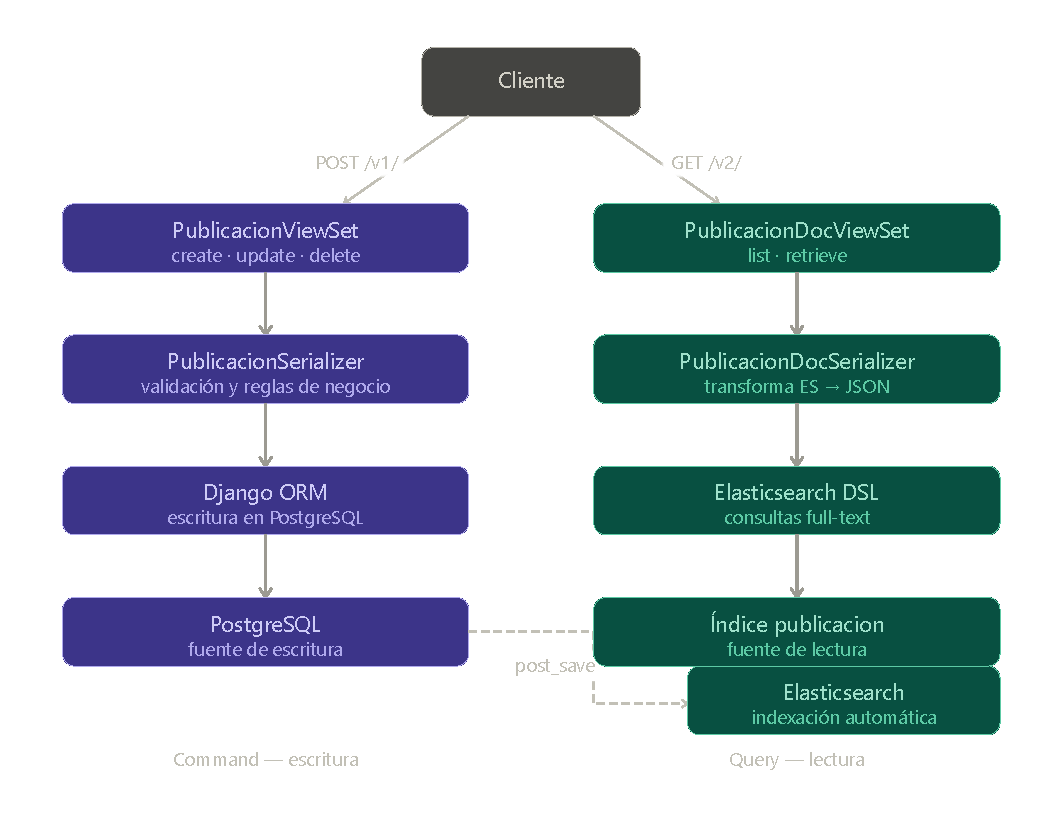
\includegraphics[width=0.95\textwidth]{Images/cqrs_picta.pdf}
  \caption{Arquitectura CQRS implementada en la API de Picta. Elaboración propia.}
  \label{fig:cqrs}
\end{figure}

\subsubsection*{\textit{Command} — camino de escritura (\texttt{/v1/publicacion/})}

El camino de escritura está implementado en \texttt{PublicacionViewSet}, que hereda de
\texttt{ModelViewSet} y expone las operaciones \texttt{create}, \texttt{update} y
\texttt{partial\_update}. Toda escritura se ejecuta dentro de una transacción atómica
(\texttt{@transaction.atomic}), garantizando la consistencia de los datos ante fallos
parciales. El \texttt{PublicacionSerializer} concentra la lógica de validación y las
reglas de negocio: verifica permisos del usuario, valida las URLs de MinIO y aplica
límites operacionales antes de persistir el registro en PostgreSQL mediante el ORM
de Django.

Una vez guardado el objeto, la señal \texttt{post\_save} de Django dispara
automáticamente la actualización del índice en Elasticsearch, manteniendo la sincronía
entre el almacén de escritura y el de lectura sin acoplar la lógica de persistencia
con la de indexación.

\subsubsection*{\textit{Query} — camino de lectura (\texttt{/v2/publicacion/})}

El camino de lectura está implementado en \texttt{PublicacionDocViewSet}, que hereda
de \texttt{DocumentViewSet} de la biblioteca \texttt{django-elasticsearch-dsl-drf}.
Este \textit{viewset} no interactúa con PostgreSQL en ningún momento: todas sus
consultas se resuelven directamente contra el índice \texttt{publicacion} de
Elasticsearch mediante la librería \texttt{elasticsearch-dsl}. El
\texttt{PublicacionDocSerializer} transforma los documentos del índice al formato
JSON esperado por el cliente, aplicando además los filtros de seguridad pertinentes
según el rol del usuario (administrador o usuario regular).

Esta separación aporta dos ventajas concretas al sistema: las consultas de búsqueda
se benefician de las capacidades de \textit{full-text search}, filtrado anidado y
paginación nativa de Elasticsearch, sin penalizar el rendimiento de escritura; y la
carga de lectura, que constituye la operación más frecuente en una plataforma de
contenido, queda completamente desacoplada del motor relacional.

\subsubsection*{Sincronización entre almacenes}

La coherencia entre PostgreSQL y Elasticsearch se mantiene a través del mecanismo
de señales de Django. Al completarse cualquier operación de escritura,
\texttt{django-elasticsearch-dsl} intercepta la señal \texttt{post\_save} del modelo
\texttt{Publicacion} e invoca \texttt{registry.update()}, que actualiza el documento
correspondiente en el índice. Este mecanismo actúa como un \textit{Observer} implícito,
desacoplando la capa de persistencia relacional de la capa de indexación sin requerir
llamadas explícitas entre ambas.

\section{Patrones de Diseño}

Los patrones de diseño son soluciones recurrentes a problemas comunes en el diseño de software a
escala de componente o clase. A diferencia de los patrones arquitectónicos, que organizan el sistema
en su conjunto, los patrones de diseño actúan a nivel de la estructura interna de los módulos. A
continuación, se describen los patrones aplicados en el desarrollo del módulo, clasificados según la
taxonomía de Gamma \citep{Gamma1994}.

\begin{enumerate}
  \item \textbf{ViewSet (Patrón de Django REST Framework):} El patrón ViewSet encapsula la lógica
  relacionada con un recurso REST en una única clase, proporcionando operaciones CRUD y acciones
  personalizadas mediante decoradores. En el módulo implementado, la clase
  \texttt{MultipartUploadViewSet} gestiona el ciclo de vida completo de una sesión de subida
  fragmentada, exponiendo las acciones \texttt{begin}, \texttt{generate\_presigned\_url},
  \texttt{add\_part}, \texttt{complete}, \texttt{cancel} y \texttt{list\_parts}. Esta
  centralización de la lógica de negocio facilita el mantenimiento y la comprensión del flujo de
  subida, agrupando en un único componente todas las operaciones sobre el recurso
  \texttt{SubidaMultipart}.

  \item \textbf{Presigned URLs (Patrón de Seguridad):} Para evitar la transmisión de credenciales
  de MinIO al frontend y permitir que el cliente suba fragmentos directamente al almacenamiento de
  objetos, se implementa el patrón de URLs prefirmadas \citep{AWS2023}. El backend genera URLs temporales firmadas
  con una validez de 2 horas que autorizan operaciones PUT específicas sobre un objeto y parte
  determinados. El método \texttt{generate\_presigned\_url} del ViewSet implementa esta lógica:

\begin{lstlisting}[language=Python, caption={Generación de URLs prefirmadas}]
@action(detail=True, methods=['get'])
def generate_presigned_url(self, request, pk=None):
    upload = self.get_object()
    part_number = int(request.query_params.get('part_number'))
    
    query_params = {
        "partNumber": str(part_number),
        "uploadId": upload.upload_id
    }
    
    url_firmada = client.get_presigned_url(
        'PUT',
        bucket_name=upload.bucket_name,
        object_name=upload.file_name,
        expires=timedelta(hours=2),
        extra_query_params=query_params
    )
    
    return Response({
        "url": url_firmada,
        "method": "PUT",
        "part_number": part_number
    })
\end{lstlisting}

  Este patrón delega la transferencia de bytes pesados directamente entre el navegador y MinIO,
  liberando al servidor Django de actuar como intermediario y reduciendo significativamente la carga
  de CPU y ancho de banda en el backend.

  \item \textbf{Validación de Permisos por Endpoint:} Cada acción del ViewSet valida que el usuario
  autenticado sea el propietario de la sesión de subida antes de autorizar la operación. Esta
  validación se implementa mediante la comparación directa \texttt{upload.owner != request.user},
  retornando un error 403 Forbidden si la condición no se cumple. Este patrón asegura que usuarios
  no autorizados no puedan manipular sesiones de subida ajenas, incluso si conocen el identificador
  de la sesión:

\begin{lstlisting}[language=Python, caption={Validación de permisos}]
upload = self.get_object()
if upload.owner != request.user:
    return Response({"error":"Forbidden"}, status=403)
\end{lstlisting}

  \item \textbf{Singleton para Cliente MinIO:} La conexión al servidor MinIO S3 se gestiona mediante
  el patrón Singleton \citep{Gamma1994}, garantizando que exista una única instancia del cliente durante todo el ciclo
  de vida de la aplicación Django. La instancia se crea mediante la función
  \texttt{crear\_cliente\_minio()} al inicio del módulo y se reutiliza en todas las operaciones del
  ViewSet:

\begin{lstlisting}[language=Python, caption={Instancia singleton del cliente MinIO}]
client = crear_cliente_minio()
\end{lstlisting}

  Dado que la creación del cliente implica el establecimiento y verificación de la conexión con el
  servidor de almacenamiento, instanciarla una sola vez reduce la latencia y el consumo de recursos
  asociados a la inicialización repetida.

  \item \textbf{Gestión de Estados mediante Modelo de Django:} El modelo \texttt{SubidaMultipart}
  persiste el estado de cada sesión de subida en la base de datos, permitiendo la reanudación tras
  interrupciones de red. Los estados posibles incluyen \texttt{in\_progress}, \texttt{completed} y
  \texttt{cancelada}. Las transiciones de estado se validan en cada endpoint:

\begin{lstlisting}[language=Python, caption={Validación de transiciones de estado}]
if upload.status == 'completed' or upload.status == 'cancelada':
    return Response({"error": "Subida culminada"},
                    status=status.HTTP_400_BAD_REQUEST)
\end{lstlisting}

  Este patrón garantiza la consistencia del estado de las sesiones y previene operaciones inválidas
  sobre subidas ya finalizadas o canceladas.

  \item \textbf{Experto en Información:} El patrón Experto en Información
  \citep{Larman2004} establece que una responsabilidad debe asignarse a la clase que
  posee la información necesaria para cumplirla. En el módulo implementado, el modelo
  \texttt{SubidaMultipart} concentra toda la información relativa a una sesión de
  carga fragmentada: el identificador de la carga (\texttt{upload\_id}), el nombre
  del objeto en MinIO (\texttt{file\_name}), el \textit{bucket} destino
  (\texttt{bucket\_name}) y las partes ya confirmadas (\texttt{parts}). En
  consecuencia, cualquier operación que requiera razonar sobre el estado de la subida
  ---como verificar si puede completarse o construir la lista de partes para el
  ensamblado final--- se delega al propio modelo, y no a la vista o a funciones
  auxiliares externas. Esto mantiene la lógica cohesionada con los datos que la
  sustentan y evita la dispersión de responsabilidades entre capas.

  \item \textbf{Controlador:} El patrón Controlador \citep{Larman2004} asigna
  la responsabilidad de recibir y coordinar los eventos del sistema a una clase que
  represente un caso de uso o un subsistema, sin ejecutar ella misma la lógica de
  negocio pesada. En la implementación, \texttt{MultipartUploadViewSet} cumple
  exactamente este rol: recibe cada solicitud HTTP, valida el estado y los permisos,
  y delega las operaciones sobre MinIO al cliente de almacenamiento y las
  persistencias al modelo. El ViewSet no calcula ni transforma datos por sí mismo;
  actúa como coordinador que distribuye el trabajo entre los componentes especializados.
  Esta separación mantiene las vistas delgadas (\textit{thin controllers}) y concentra
  la lógica de dominio en el modelo, en línea con las convenciones de Django REST
  Framework.
\end{enumerate}

\section{Conclusiones Parciales}

La propuesta de solución define un módulo de carga fragmentada que integra seis funcionalidades 
fundamentales ---gestión de estados, pausa arbitraria, reanudación desde el último fragmento, 
persistencia histórica, procesamiento diferido de metadatos y listado de videos pendientes--- 
orientadas al rol de administrador de canal. El análisis del modelo de usuarios sustentó la 
delimitación del alcance mediante la herencia de permisos existente en Django, garantizando una 
integración \textit{seamless} con la arquitectura de autorización en producción.

La especificación de requisitos mediante historias de usuario bajo el marco Scrum permitió 
formalizar las expectativas del cliente en términos de funcionalidades verificables. La estimación 
de esfuerzo resultó en un total de 36 puntos de historia distribuidos en tres sprints de dos 
semanas, estableciendo un plan de entrega que equilibra la complejidad técnica del backend ---subida 
multipart, generación de URLs prefirmadas, validación de checksums--- con el desarrollo de 
componentes reactivos en el frontend Angular.

La adopción de la arquitectura dirigida por eventos como patrón arquitectónico central desacopla la 
subida de la transcodificación, mientras que los patrones de diseño implementados ---ViewSet para 
encapsular la lógica REST, Presigned URLs para delegar la transferencia directa a MinIO, validación 
de permisos por endpoint y Singleton para el cliente de almacenamiento--- constituyen decisiones 
técnicas orientadas a reducir la carga del servidor, fortalecer la seguridad y garantizar la 
persistencia del estado ante interrupciones de red.